\clearpage
\section{Результаты вычислительного эксперимента}
	Архитектуры нейронных сетей, а также модификация процедуры обучения, описанные в пунктах 1.4.3 и 1.4.4 были реализованы в виде комплекса программ на языке Python с помощью библиотеки для глубокого обучения PyTorch. Использованные версии программных пакетов указаны в Приложении 1. Обучение проводилось на наборе данных Berea.
	
	\subsection{Набор данных Berea}
		Исходные данные - изображение компьютерной томографии песчаника, объёмом $400^3$ вокселей, бинарно сегментированная на породу и поры, в формате TIFF. Разрешение томограммы равно 3 микрометрам. Для обучения сетей из этого кубика был вырезан набор кубиков размером $64^3$ вокселей, с перекрытием в 16 вокселей (всего 10648 различных образцов размера $64^3$), они и представили собой обучающую выборку. Оригинальный образец размером $400^3$ вокселей представлен на (Рис. \ref{5-full-berea}). Некоторые примеры из получившейся обучающей выборки представлены в (Таб. \ref{5-berea64}).
		
		\begin{figure}[h]
			\centering{\includegraphics[width=0.6\linewidth]{5-results/berea/original}}
			\caption{Оригинальный образец}
			\label{5-full-berea}
		\end{figure}
	
		\begin{table}[h]
			\centering
			\begin{tabular}{p{5cm} p{5cm} p{5cm}}
				\toprule
				\includegraphics[width=1.0\linewidth]{5-results/berea/berea_1}
				&
				\includegraphics[width=1.0\linewidth]{5-results/berea/berea_2}
				&
				\includegraphics[width=1.0\linewidth]{5-results/berea/berea_3}
				\\
				\includegraphics[width=1.0\linewidth]{5-results/berea/berea_4}
				&
				\includegraphics[width=1.0\linewidth]{5-results/berea/berea_5}
				&
				\includegraphics[width=1.0\linewidth]{5-results/berea/berea_6}
				\\
				\bottomrule
			\end{tabular}
			\caption{Примеры из обучающей выборки}
			\label{5-berea64}
		\end{table}
	\subsection{Обучение нейросети}
		Было проведено обучение нейросети со следующими параметрами (число свёрточных фильтров указано для первого слоя):
		\begin{table}[h]
			\centering
			\begin{tabular}{|c|c|c|c|}
				\hline
				Число фильтров G, D & Размерность z & Размер пакета & Начальный LR \\
				\hline
				64, 32 & 512 & 64 & 2e-4 \\
				\hline
			\end{tabular}
			\caption{Гиперпараметры нейросети и процесса обучения}
		\end{table}
	
		Итоговые архитектуры использованных нейронных сетей генератора и дискриминатора указаны в (Таб. \ref{5-g-arch}, \ref{5-d-arch})
		\begin{table}[h]
			\tabcolsep=0.11cm
			\centering
			\begin{tabular}{|c|c|c|c|}
				\hline
				Слой & Размер ядра & Размерность выхода & Кол-во параметров \\
				\hline
				0\_ConvTranspose3d &  [256, 512, 4, 4, 4] & [1, 256, 4, 4, 4] & 8 388 610 \\
				1\_BatchNorm3d &  [256] & [1, 256, 4, 4, 4] & 512 \\
				2\_ReLU & - & [1, 256, 4, 4, 4] & - \\
				\hline
				3\_ConvTranspose3d &  [128, 256, 4, 4, 4] & [1, 128, 8, 8, 8] & 2 097 150 \\
				4\_BatchNorm3d &  [128] & [1, 128, 8, 8, 8] & 256 \\
				5\_ReLU & - & [1, 128, 8, 8, 8] & - \\
				\hline
				6\_ConvTranspose3d &  [64, 128, 4, 4, 4] & [1, 64, 16, 16, 16] & 524 290 \\
				7\_BatchNorm3d &  [64] & [1, 64, 16, 16, 16] & 128 \\
				8\_ReLU & - & [1, 64, 16, 16, 16] & - \\
				\hline
				9\_ConvTranspose3d &  [32, 64, 4, 4, 4] & [1, 32, 32, 32, 32] & 131 070 \\
				10\_BatchNorm3d &  [32] & [1, 32, 32, 32, 32] & 64 \\
				11\_ReLU & - & [1, 32, 32, 32, 32] & - \\
				\hline
				12\_ConvTranspose3d &  [1, 32, 4, 4, 4] & [1, 1, 64, 64, 64] & 2 050 \\
				13\_Tanh & - & [1, 1, 64, 64, 64] & - \\
				\hline
			\end{tabular}
			\caption{Архитектура генератора}
			\label{5-g-arch}
		\end{table}
	
		\begin{table}[h]
			\tabcolsep=0.11cm
			\centering
			\begin{tabular}{|c|c|c|c|}
				\hline
				Слой & Размер ядра & Размерность выхода & Кол-во параметров \\
				\hline
				0\_Conv3d &  [1, 32, 4, 4, 4] & [1, 32, 32, 32, 32] & 2 050 \\
				1\_LeakyReLU & - & [1, 32, 32, 32, 32] & - \\
				\hline
				2\_Conv3d &  [32, 64, 4, 4, 4] & [1, 64, 16, 16, 16] & 131 070 \\
				3\_BatchNorm3d &  [64] & [1, 64, 16, 16, 16] & 128 \\
				4\_LeakyReLU & - & [1, 64, 16, 16, 16] & - \\
				\hline
				5\_Conv3d &  [64, 128, 4, 4, 4] & [1, 128, 8, 8, 8] & 524 290 \\
				6\_BatchNorm3d &  [128] & [1, 128, 8, 8, 8] & 256 \\
				7\_LeakyReLU & - & [1, 64, 16, 16, 16] & - \\
				\hline
				8\_Conv3d &  [128, 256, 4, 4, 4] & [1, 256, 4, 4, 4] & 2 097 150 \\
				9\_BatchNorm3d &  [256] & [1, 256, 4, 4, 4] & 512 \\
				10\_LeakyReLU & - & [1, 256, 4, 4, 4] & - \\
				\hline
				11\_Conv3d &  [256, 1, 4, 4, 4] & [1, 1, 1, 1, 1] & 16 380 \\
				12\_Sigmoid & - & [1, 1, 1, 1, 1] & - \\
				\hline
			\end{tabular}
			\caption{Архитектура дискриминатора}
			\label{5-d-arch}
		\end{table}
		
		Графики функций ошибок сетей генератора и дискриминатора, а также графики сходимостей функционалов Минковского в процессе обучения приведены на (Рис. \ref{loss-plot}, \ref{V-plot}, \ref{S-plot}, \ref{B-plot}, \ref{Xi-plot}).
		
		\begin{figure}[h]
			\centering{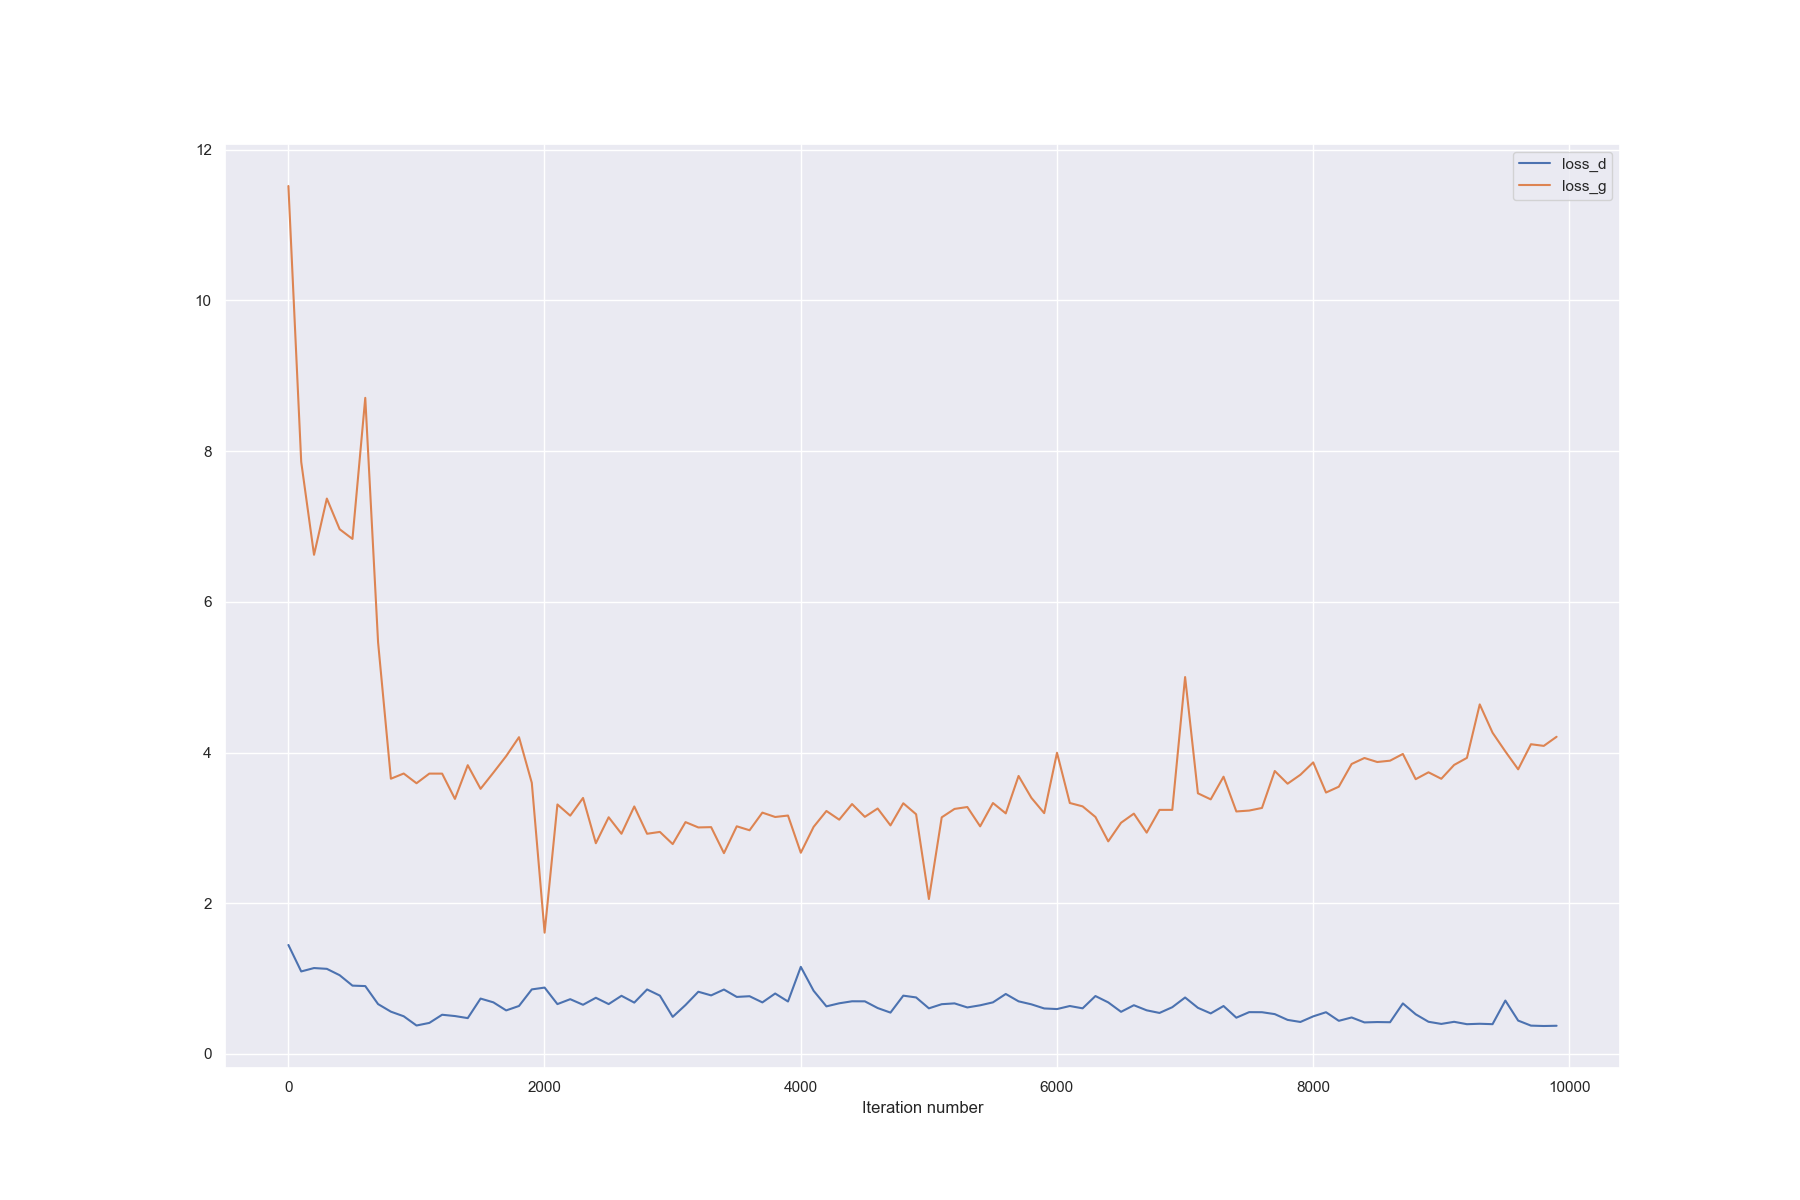
\includegraphics[width=0.95\linewidth]{5-results/experiment/loss_plot}}
			\caption{График функций ошибок сетей дискриминатора и генератора}
			\label{loss-plot}
		\end{figure}
	
		\begin{figure}[h]
			\centering{\includegraphics[width=0.95\linewidth]{5-results/experiment/minkowski_V_plot}}
			\caption{График сходимости функционала Минковского $V$}
			\label{V-plot}
		\end{figure}
		
		\begin{figure}[h]
			\centering{\includegraphics[width=0.95\linewidth]{5-results/experiment/minkowski_S_plot}}
			\caption{График сходимости функционала Минковского $S$}
			\label{S-plot}
		\end{figure}
	
		\begin{figure}[h]
			\centering{\includegraphics[width=0.95\linewidth]{5-results/experiment/minkowski_B_plot}}
			\caption{График сходимости функционала Минковского $B$}
			\label{B-plot}
		\end{figure}
	
		\begin{figure}[h]
			\centering{\includegraphics[width=0.95\linewidth]{5-results/experiment/minkowski_Xi_plot}}
			\caption{График сходимости функционала Минковского $\xi$}
			\label{Xi-plot}
		\end{figure}	
		
	
	\subsection{Реконструкции размера $64^3$}
		\subsubsection{Примеры}
			Примеры реконструкций размера $64^3$, приведены в (Таб. \ref{5-gen-64}). Дополнительные примеры реконструкций приведены в Приложении 2 (Таб. \ref{8-gen-64}).
			
			\begin{table}[h]
				\centering
				\begin{tabular}{p{5cm} p{5cm} p{5cm}}
					\toprule
					\includegraphics[width=1\linewidth]{5-results/analysis_64/generated/1}
					&
					\includegraphics[width=1\linewidth]{5-results/analysis_64/generated/2}
					&
					\includegraphics[width=1\linewidth]{5-results/analysis_64/generated/3}
					\\
					\includegraphics[width=1\linewidth]{5-results/analysis_64/generated/4}
					&
					\includegraphics[width=1\linewidth]{5-results/analysis_64/generated/5}
					&
					\includegraphics[width=1\linewidth]{5-results/analysis_64/generated/6}
					\\
					\includegraphics[width=1\linewidth]{5-results/analysis_64/generated/7}
					&
					\includegraphics[width=1\linewidth]{5-results/analysis_64/generated/8}
					&
					\includegraphics[width=1\linewidth]{5-results/analysis_64/generated/9}
					\\
					\bottomrule
				\end{tabular}
				\caption{Примеры реконструкций 64x64x64}
				\label{5-gen-64}
			\end{table} 
		
		\subsubsection{Анализ реконструкций}
			Было реконструировано 1000 образцов размера $64^3$. На основе этого набора были получены распределения интересующих функционалов Минковского. Также, используя предоставленную обученную сеть \cite{Mosser}, было реконструировано 1000 образцов того же размера для сравнения распределений функционалов. Графики полученных распределений (вместе с соответствующим распределением на обучающей выборке) приведены на (Рис. \ref{5-dist-V-64}, \ref{5-dist-S-64}, \ref{5-dist-B-64}, \ref{5-dist-Xi-64}). Была рассчитана двухточечная функция вероятности для реконструированных образцов, образцов, полученных с помощью предобученной сети \cite{Mosser} и образцов из обучающей выборки. Её график приведён на (Рис. \ref{5-prob-64}).
			
			\begin{figure}[h]
				\begin{minipage}[h]{0.49\linewidth}
					\centering{\includegraphics[width=1\linewidth]{5-results/analysis_64/V_exp} \\ Обученная сеть}
				\end{minipage}
				\hfill
				\begin{minipage}[h]{0.49\linewidth}
					\centering{\includegraphics[width=1\linewidth]{5-results/analysis_64/V_paper} \\ Mosser et al. \cite{Mosser}}
				\end{minipage}
				\caption{Распределения функционала Минковского $V$ для реконструкций размера $64^3$}
				\label{5-dist-V-64}
			\end{figure}
		
			\begin{figure}[h]
				\begin{minipage}[h]{0.49\linewidth}
					\centering{\includegraphics[width=1\linewidth]{5-results/analysis_64/S_exp} \\ Обученная сеть}
				\end{minipage}
				\hfill
				\begin{minipage}[h]{0.49\linewidth}
					\centering{\includegraphics[width=1\linewidth]{5-results/analysis_64/S_paper} \\ Mosser et al. \cite{Mosser}}
				\end{minipage}
				\caption{Распределения функционала Минковского $S$ для реконструкций размера $64^3$}
				\label{5-dist-S-64}
			\end{figure}
		
			\begin{figure}[h]
				\begin{minipage}[h]{0.49\linewidth}
					\centering{\includegraphics[width=1\linewidth]{5-results/analysis_64/B_exp} \\ Обученная сеть}
				\end{minipage}
				\hfill
				\begin{minipage}[h]{0.49\linewidth}
					\centering{\includegraphics[width=1\linewidth]{5-results/analysis_64/B_paper} \\ Mosser et al. \cite{Mosser}}
				\end{minipage}
				\caption{Распределения функционала Минковского $B$ для реконструкций размера $64^3$}
				\label{5-dist-B-64}
			\end{figure}
		
			\begin{figure}[h]
				\begin{minipage}[h]{0.49\linewidth}
					\centering{\includegraphics[width=1\linewidth]{5-results/analysis_64/Xi_exp} \\ Обученная сеть}
				\end{minipage}
				\hfill
				\begin{minipage}[h]{0.49\linewidth}
					\centering{\includegraphics[width=1\linewidth]{5-results/analysis_64/Xi_paper} \\ Mosser et al. \cite{Mosser}}
				\end{minipage}
				\caption{Распределения функционала Минковского $\xi$ для реконструкций размера $64^3$}
				\label{5-dist-Xi-64}
			\end{figure}
		
			\begin{figure}[h]
				\begin{minipage}[h]{0.49\linewidth}
					\centering{\includegraphics[width=1\linewidth]{5-results/analysis_64/prob_exp} \\ Обученная сеть}
				\end{minipage}
				\hfill
				\begin{minipage}[h]{0.49\linewidth}
					\centering{\includegraphics[width=1\linewidth]{5-results/analysis_64/prob_paper} \\ Mosser et al. \cite{Mosser}}
				\end{minipage}
				\caption{Двухточечная функция вероятности для реконструкций размера $64^3$}
				\label{5-prob-64}
			\end{figure}
	
	\subsection{Реконструкции размера $216^3$}
		\subsubsection{Примеры}
			Примеры реконструкций размера $216^3$, приведены в (Таб. \ref{5-gen-216}). Дополнительные примеры реконструкций приведены в Приложении 2 (Таб. \ref{8-gen-216}).
		
			\begin{table}[h]
				\centering
				\begin{tabular}{p{5cm} p{5cm} p{5cm}}
					\toprule
					\includegraphics[width=1\linewidth]{5-results/analysis_216/generated/1}
					&
					\includegraphics[width=1\linewidth]{5-results/analysis_216/generated/2}
					&
					\includegraphics[width=1\linewidth]{5-results/analysis_216/generated/3}
					\\
					\includegraphics[width=1\linewidth]{5-results/analysis_216/generated/4}
					&
					\includegraphics[width=1\linewidth]{5-results/analysis_216/generated/5}
					&
					\includegraphics[width=1\linewidth]{5-results/analysis_216/generated/6}
					\\
					\includegraphics[width=1\linewidth]{5-results/analysis_216/generated/7}
					&
					\includegraphics[width=1\linewidth]{5-results/analysis_216/generated/8}
					&
					\includegraphics[width=1\linewidth]{5-results/analysis_216/generated/9}
					\\
					\bottomrule
				\end{tabular}
				\caption{Примеры реконструкций 216x216x216}
				\label{5-gen-216}
			\end{table} 
		
		\subsubsection{Анализ реконструкций}
			Было реконструировано 500 образцов размера $216^3$. На основе этого набора были получены распределения интересующих функционалов Минковского. Также, используя предоставленную обученную сеть \cite{Mosser}, было реконструировано 500 образцов того же размера для сравнения распределений функционалов. Графики полученных распределений приведены на (Рис. \ref{5-dist-V-216}, \ref{5-dist-S-216}, \ref{5-dist-B-216}, \ref{5-dist-Xi-216}). Была рассчитана двухточечная функция вероятности для реконструированных образцов, образцов, полученных с помощью предобученной сети \cite{Mosser} и образцов из обучающей выборки. Её график приведён на (Рис. \ref{5-prob-216}).
		
			\begin{figure}[h]
				\begin{minipage}[h]{0.49\linewidth}
					\centering{\includegraphics[width=1\linewidth]{5-results/analysis_216/V_exp} \\ Обученная сеть}
				\end{minipage}
				\hfill
				\begin{minipage}[h]{0.49\linewidth}
					\centering{\includegraphics[width=1\linewidth]{5-results/analysis_216/V_paper} \\ Mosser et al. \cite{Mosser}}
				\end{minipage}
				\caption{Распределения функционала Минковского $V$ для реконструкций размера $216^3$}
				\label{5-dist-V-216}
			\end{figure}
			
			\begin{figure}[h]
				\begin{minipage}[h]{0.49\linewidth}
					\centering{\includegraphics[width=1\linewidth]{5-results/analysis_216/S_exp} \\ Обученная сеть}
				\end{minipage}
				\hfill
				\begin{minipage}[h]{0.49\linewidth}
					\centering{\includegraphics[width=1\linewidth]{5-results/analysis_216/S_paper} \\ Mosser et al. \cite{Mosser}}
				\end{minipage}
				\caption{Распределения функционала Минковского $S$ для реконструкций размера $216^3$}
				\label{5-dist-S-216}
			\end{figure}
			
			\begin{figure}[h]
				\begin{minipage}[h]{0.49\linewidth}
					\centering{\includegraphics[width=1\linewidth]{5-results/analysis_216/B_exp} \\ Обученная сеть}
				\end{minipage}
				\hfill
				\begin{minipage}[h]{0.49\linewidth}
					\centering{\includegraphics[width=1\linewidth]{5-results/analysis_216/B_paper} \\ Mosser et al. \cite{Mosser}}
				\end{minipage}
				\caption{Распределения функционала Минковского $B$ для реконструкций размера $216^3$}
				\label{5-dist-B-216}
			\end{figure}
			
			\begin{figure}[h]
				\begin{minipage}[h]{0.49\linewidth}
					\centering{\includegraphics[width=1\linewidth]{5-results/analysis_216/Xi_exp} \\ Обученная сеть}
				\end{minipage}
				\hfill
				\begin{minipage}[h]{0.49\linewidth}
					\centering{\includegraphics[width=1\linewidth]{5-results/analysis_216/Xi_paper} \\ Mosser et al. \cite{Mosser}}
				\end{minipage}
				\caption{Распределения функционала Минковского $\xi$ для реконструкций размера $216^3$}
				\label{5-dist-Xi-216}
			\end{figure}
		
			\begin{figure}[h]
				\begin{minipage}[h]{0.49\linewidth}
					\centering{\includegraphics[width=1\linewidth]{5-results/analysis_216/prob_exp} \\ Обученная сеть}
				\end{minipage}
				\hfill
				\begin{minipage}[h]{0.49\linewidth}
					\centering{\includegraphics[width=1\linewidth]{5-results/analysis_216/prob_paper} \\ Mosser et al. \cite{Mosser}}
				\end{minipage}
				\caption{Двухточечная функция вероятности для реконструкций размера $216^3$}
				\label{5-prob-216}
			\end{figure}

	\subsection{Реконструкции размера $360^3$}
		\subsubsection{Примеры}
			Примеры реконструкций размера $360^3$, приведены в (Таб. \ref{5-gen-360}). Дополнительные примеры реконструкций приведены в Приложении 2 (Таб. \ref{8-gen-360}).
			
			\begin{table}[h]
				\centering
				\begin{tabular}{p{5cm} p{5cm} p{5cm}}
					\toprule
					\includegraphics[width=1\linewidth]{5-results/analysis_360/generated/1}
					&
					\includegraphics[width=1\linewidth]{5-results/analysis_360/generated/2}
					&
					\includegraphics[width=1\linewidth]{5-results/analysis_360/generated/3}
					\\
					\includegraphics[width=1\linewidth]{5-results/analysis_360/generated/4}
					&
					\includegraphics[width=1\linewidth]{5-results/analysis_360/generated/5}
					&
					\includegraphics[width=1\linewidth]{5-results/analysis_360/generated/6}
					\\
					\includegraphics[width=1\linewidth]{5-results/analysis_360/generated/7}
					&
					\includegraphics[width=1\linewidth]{5-results/analysis_360/generated/8}
					&
					\includegraphics[width=1\linewidth]{5-results/analysis_360/generated/9}
					\\
					\bottomrule
				\end{tabular}
				\caption{Примеры реконструкций 360x360x360}
				\label{5-gen-360}
			\end{table} 
	
		\subsubsection{Анализ реконструкций}
			Было реконструировано 500 образцов размера $360^3$. На основе этого набора были получены распределения интересующих функционалов Минковского. Также, используя предоставленную обученную сеть \cite{Mosser}, было реконструировано 1000 образцов того же размера для сравнения распределений функционалов. Графики полученных распределений приведены на (Рис. \ref{5-dist-V-360}, \ref{5-dist-S-360}, \ref{5-dist-B-360}, \ref{5-dist-Xi-360}). Была рассчитана двухточечная функция вероятности для реконструированных образцов, образцов, полученных с помощью предобученной сети \cite{Mosser} и образцов из обучающей выборки. Её график приведён на (Рис. \ref{5-prob-360}).
			
			\begin{figure}[h]
				\begin{minipage}[h]{0.49\linewidth}
					\centering{\includegraphics[width=1\linewidth]{5-results/analysis_360/V_exp} \\ Обученная сеть}
				\end{minipage}
				\hfill
				\begin{minipage}[h]{0.49\linewidth}
					\centering{\includegraphics[width=1\linewidth]{5-results/analysis_360/V_paper} \\ Mosser et al. \cite{Mosser}}
				\end{minipage}
				\caption{Распределения функционала Минковского $V$ для реконструкций размера $360^3$}
				\label{5-dist-V-360}
			\end{figure}
			
			\begin{figure}[h]
				\begin{minipage}[h]{0.49\linewidth}
					\centering{\includegraphics[width=1\linewidth]{5-results/analysis_360/S_exp} \\ Обученная сеть}
				\end{minipage}
				\hfill
				\begin{minipage}[h]{0.49\linewidth}
					\centering{\includegraphics[width=1\linewidth]{5-results/analysis_360/S_paper} \\ Mosser et al. \cite{Mosser}}
				\end{minipage}
				\caption{Распределения функционала Минковского $S$ для реконструкций размера $360^3$}
				\label{5-dist-S-360}
			\end{figure}
			
			\begin{figure}[h]
				\begin{minipage}[h]{0.49\linewidth}
					\centering{\includegraphics[width=1\linewidth]{5-results/analysis_360/B_exp} \\ Обученная сеть}
				\end{minipage}
				\hfill
				\begin{minipage}[h]{0.49\linewidth}
					\centering{\includegraphics[width=1\linewidth]{5-results/analysis_360/B_paper} \\ Mosser et al. \cite{Mosser}}
				\end{minipage}
				\caption{Распределения функционала Минковского $B$ для реконструкций размера $360^3$}
				\label{5-dist-B-360}
			\end{figure}
			
			\begin{figure}[h]
				\begin{minipage}[h]{0.49\linewidth}
					\centering{\includegraphics[width=1\linewidth]{5-results/analysis_360/Xi_exp} \\ Обученная сеть}
				\end{minipage}
				\hfill
				\begin{minipage}[h]{0.49\linewidth}
					\centering{\includegraphics[width=1\linewidth]{5-results/analysis_360/Xi_paper} \\ Mosser et al. \cite{Mosser}}
				\end{minipage}
				\caption{Распределения функционала Минковского $\xi$ для реконструкций размера $360^3$}
				\label{5-dist-Xi-360}
			\end{figure}
		
			\begin{figure}[h]
				\begin{minipage}[h]{0.49\linewidth}
					\centering{\includegraphics[width=1\linewidth]{5-results/analysis_360/prob_exp} \\ Обученная сеть}
				\end{minipage}
				\hfill
				\begin{minipage}[h]{0.49\linewidth}
					\centering{\includegraphics[width=1\linewidth]{5-results/analysis_360/prob_paper} \\ Mosser et al. \cite{Mosser}}
				\end{minipage}
				\caption{Двухточечная функция вероятности для реконструкций размера $360^3$}
				\label{5-prob-360}
			\end{figure}
			
		%\begin{figure}[h]
		%	\begin{minipage}[h]{0.49\linewidth}
		%		\centering{\includegraphics[width=1\linewidth]{5-results/analysis_360/corr_exp} \\ Обученная сеть}
		%	\end{minipage}
		%	\hfill
		%	\begin{minipage}[h]{0.49\linewidth}
		%		\centering{\includegraphics[width=1\linewidth]{5-results/analysis_360/corr_paper} \\ Mosser et al. \cite{Mosser}}
		%	\end{minipage}
		%	\caption{Двухточечная функция корреляции для реконструкций размера $360^3$}
		%	\label{5-corr-360}
		%\end{figure}